%preamble
\documentclass[letterpaper]{article}
\synctex=1
\usepackage{graphicx}
\graphicspath{ {images/} }

\usepackage{lipsum}
\usepackage{float}

\usepackage{amssymb}

\usepackage{siunitx}

\usepackage{multirow}
% for merging table cells I think

\usepackage{tabularx}
\renewcommand\tabularxcolumn[1]{m{#1}}% for vertical centering text in X column

% allows for linewrap within cells
\newcolumntype{Y}{>{\centering\arraybackslash}X}

\usepackage{todonotes}
\usepackage{hyperref}

\usepackage{pdfpages} % for attaching the table lol

\title{ECE 322 \\
Lab Report 1}
\author{Arun Woosaree\\
XXXXXXX}
\begin{document}
\maketitle

\section*{Introduction}
The purpose of this lab was to serve as a practical introduction to rudimentary black-box testing techniques.
The testing methods introduced were dirty testing, error guessing, and partition-based testing.
It should be noted that numerous other black-box testing methods exist
The idea of black-box testing is that tests are carried out with no knowledge of how the software
internally works. In other words, the implementation details are a ``black box'' as the name would suggest.
Dirty testing and error guessing involves using creativity to come up with test cases,
and also using past experiences to come up with test cases to find faults in the program.
The purpose of partition-based testing is to categorize possible test cases in `equivalence'
classes, and to test as many valid equivalence classes with as few test cases, and to come up
with a test case for each invalid equivalence class. The goal for partition-based testing
is to lower the number of test cases.

\section*{Part 1 - Failure/Dirty Testing, Error Guessing}
For task one in this lab, we had to be creative, as is the nature of Failure/Dirty testing, and error guessing.
The purpose was to test the functionality of a calculator program, which was written in Java. A table of
test cases was produced, checking for basic functionality, common errors. A few test cases were also
made based on previous experience, which is also known as error guessing. Altogether, the test cases check
for the following functionality:

\begin{enumerate}
    \item whether the calculator buttons work
    \item non-numerical input
    \item mismatched brackets
    \item order or operations (BEDMAS/PEMDAS)
    \item large numbers
    \item small numbers
    \item incorrect syntax (e.g. 2++2)
\end{enumerate}

The full list of test cases, along with the inputs and expected versus actual outputs can be found in Appendix \ref{calculatortestcases}.
The test cases where the expected result does not match the actual result are highlighted in red.
From experience, these test failures could be due to the following:
\begin{itemize}
    \item numbers like $2^{512}$ are ridiculously big. It's likely that that the implementation was not designed to handle such large numbers.
    \item similarly, numbers like $2^{-512}$ are so small that the calculator interprets it as being the number 0
    \item entering nothing results in an output of 0. It's likely that a lone space is interpreted as a 0 by the calculator
    \item if there's a space between a number and the minus sign after it, the calculator outputs NaN. It could be that when parsing the input, the calculator may be interpreting it as two numbers with no operator in between, so it does not know what to do and returns an error (NaN)
    \item the calculator does not follow the correct order of operations.
          If there's a division and multiplication. (e.g. $80/4*5$),
          it appears to be doing the multiplication before the division,
          even though the multiplication should be done afterwards,
          since it is on the right hand side of the previous division operation.
    \item when multiple exponent (\textasciicircum) operators are used in between two operands,
          the result is always one, instead of showing an error. This might be because the right half is evaluated as 0 by the calculator,
          and anything to the power of 0 is 1.
    \item when the first operand is missing for $+$ the calculator seems to ignore it and treat it like a positive number. This is why the calculator says $2++++2=4$
    \item when the first operand is missing for $*$, $/$, or \textasciicircum, the calculator evaluates it as being equal to 0 instead of returning an error.
          % This becomes apparent in operations like $\textrm2$,  $2**2$, or $/2$
    \item with the exponent operator, the calculator tries to evaluate everything after the exponent.
          however, this violates the BEDMAS rule in cases where the exponent should be done before multiplication, division, addition, or subtraction.
          This results in errors like $2^1+1$ resulting in 4 instead of 3.
          This also compounds with the previous errors in some cases where an expression like $2^3 + 2^3$
          is incorrectly evaluated as $2^5$, since $3+2$ is evaluated first, which results in 
          \textasciicircum 3
          being evaluated as 1, and the expression is reduced to $2^{5}$, resulting in the incorrect response.
    \item when numbers are only separated by a space, the calculator concatenates the digits. i.e. 1 2 becomes 12, instead of showing an error.
          when these numbers are wrapped by brackets, the calculator still concatenates them instead of multiplying. e.g. (2)(2) becomes 22 instead of 4.
          However, multiplying negative numbers using brackets e.g. (2)(-2) instead of the * operator results in a NaN error.
    \item the calculator has some rounding issues, which result in a loss of precision in the answer. Adding numbers like $2.000001+2.000002$ result in a rounded
          answer instead of the exact answer.
\end{itemize}
% \todo{fix the table and highlightthe failed test case}

\section*{Part 2 - Partition Testing}
Task two of this lab involved partition-based testing of a triangle application.
The purpose of this application is to take 3 space separated positive integers,
each representing sides of a triangle, and the program is expected to tell the
user whether the triangle is a scalene, isosceles, or equilateral triangle.
The following equivalence classes were decided on for creating the test cases.
\subsection*{Triangle Equivalence Classes}

\begin{table}[H]
    \begin{tabularx}{1.1\textwidth}{X|X|X|}
        \centering
        Input Condition                       & Valid Input Classes   & Invalid Input Classes                         \\ \hline
        number of input arguments             & 3 input arguments (1) & $< 3$ input arguments (9)                     \\
                                              &                       & $> 3$ input arguments (10)                    \\ \hline
        space between arguments               & one space (2)         & more than one space (11)                      \\
                                              &                       & non space character separating arguments (12) \\ \hline
        argument type                         & positive integer (3)  & negative integer (13)                         \\
                                              &                       & zero (14)                                     \\
                                              &                       & decimal (15)                                  \\ \hline
        triangle type                         & equilateral (4)       & $a + b = c$ (16)                              \\
                                              & isosceles (5)         & $a + b < c$ (17)                              \\
                                              & scalene (6)           &                                               \\
                                              & $a + b > c$ (7)       &                                               \\ \hline
        key pressed after inputting arguments & Enter key pressed (8) & Enter key not pressed (18)                    \\ \hline
    \end{tabularx}
    \caption{Valid and Invalid equivalence classes for the triangle program}
    \label{equivalenceclasses}
\end{table}

From these equivalence classes, the following test cases were created:

\subsection*{Test cases for valid inputs}
\begin{itemize}
    \item 3 3 3 covers (1, 2, 3, 4, 7, 8)
    \item 4 4 5 covers (1, 2, 3, 5, 7, 8)
    \item 6 7 8 covers (1, 2, 3, 6, 7, 8)
\end{itemize}

\subsection*{Test cases for invalid inputs}
\begin{itemize}
    \item 1 2 covers (9)
    \item 3 4 5 6 covers (10)
    \item 7 8 \qquad 9 covers (11)
    \item 8\_7\_6 covers (12)
    \item 1 $-2$ 3 covers (13)
    \item 5 0 4 covers (14)
    \item 3 2 0.1 covers (15)
    \item 2 2 4 covers (16)
    \item 3 4 9 covers (17)
    \item not pressing Enter covers (18)
\end{itemize}

The results of these test cases, including expected versus actual output can be found in Appendix \ref{triangletestcases}.
Failed test cases are highlighted in red. There was one test case which failed. 

\begin{itemize}
    \item For the input where we have the case $a+b=c$,
    (2 2 4) in this case, the program tells us that it is a isosceles triangle instead of an invalid one.
    This is likely because the implementation checks validity by looking for $a+b>c$ instead of $a+b \geq c$.    
    Similarly, with the inputs (1 2 3), the program tells us that it is a scalene triangle instead of showing an error.
\end{itemize}

\section*{Conclusion}
In this lab, we were introduced to black-box testing. The techniques
learned were dirty testing, error guessing, and partition-based testing.
Dirty testing's strength seems to also be its weakness at the same time. That is,
the test cases written are only limited by the tester's creativity.
One disadvantage, however, is that one can generate a lot of extra test cases
that are arguably unnecessary. That is, there is the possibility of having multiple
tests which cover the same functionality of the program. This is a problem that
using the partition-based testing method addressed. While equivalence testing allowed us 
to write significantly fewer test cases,
it does not catch some unique cases. For example, if dirty testing was done instead,
one might have tried the test inputs $$1111111111\ 1111111111\ 1$$, which returns ERROR: Invalid triangle
instead of saying that it's an isosceles one. This error, and potentially others were not
caught using partition-based testing. What is interesting, though is that the one
test failure with inputs (2 2 4) for the Triangle program allowed for another error to be found, which is
the case where an input like (1 2 3) which should cause an error instead returns `Scalene'.
Overall, it would not be fair to say that
one testing method is universally better than the other, however, the tester would
need to use their judgement and experience to choose an appropriate testing method
for the software that they want to test.

\appendix
\section*{Appendix}
\section{Calculator Test Cases} \label{calculatortestcases}
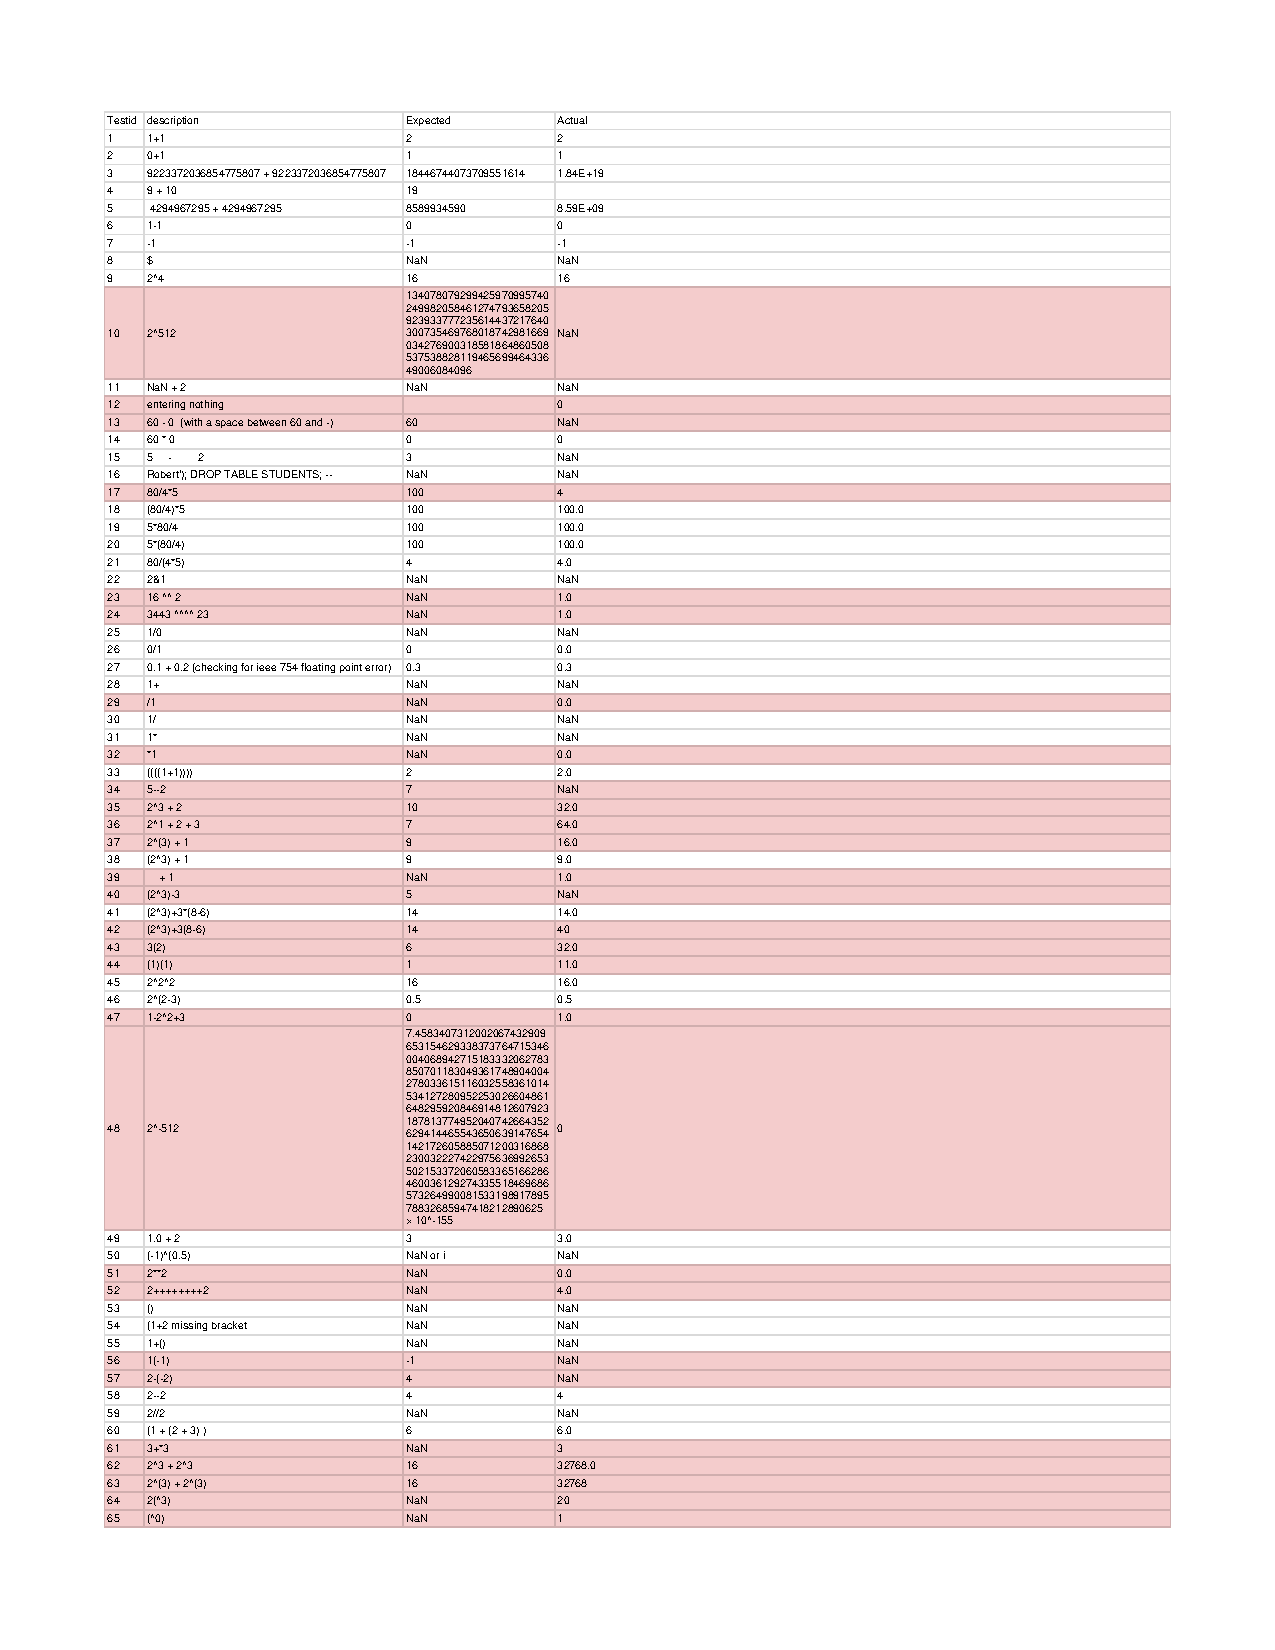
\includepdf[pages=-]{calculatortable.pdf}

\section{Triangle Test Cases} \label{triangletestcases}
% 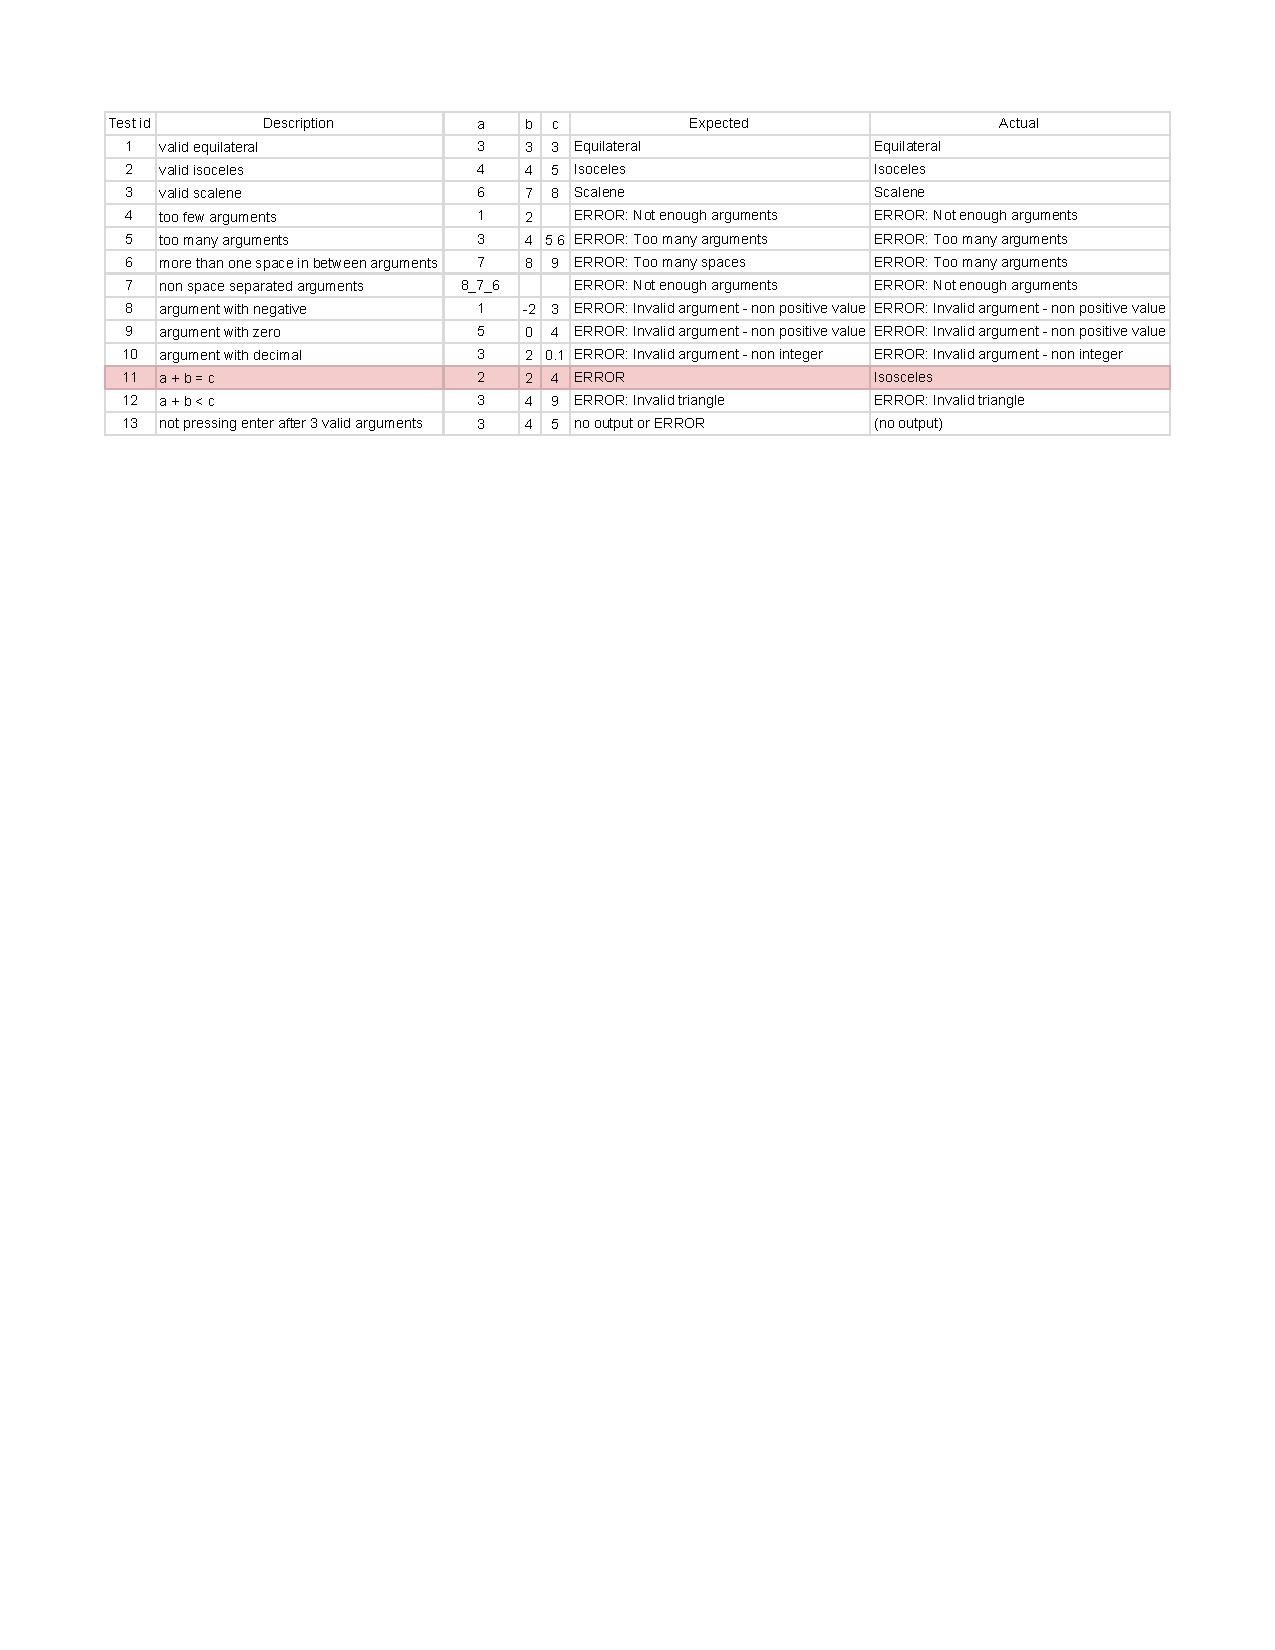
\includepdf[]{triangletable.pdf}
\begin{table}[H]
    \begin{figure}[H]
        \centering
        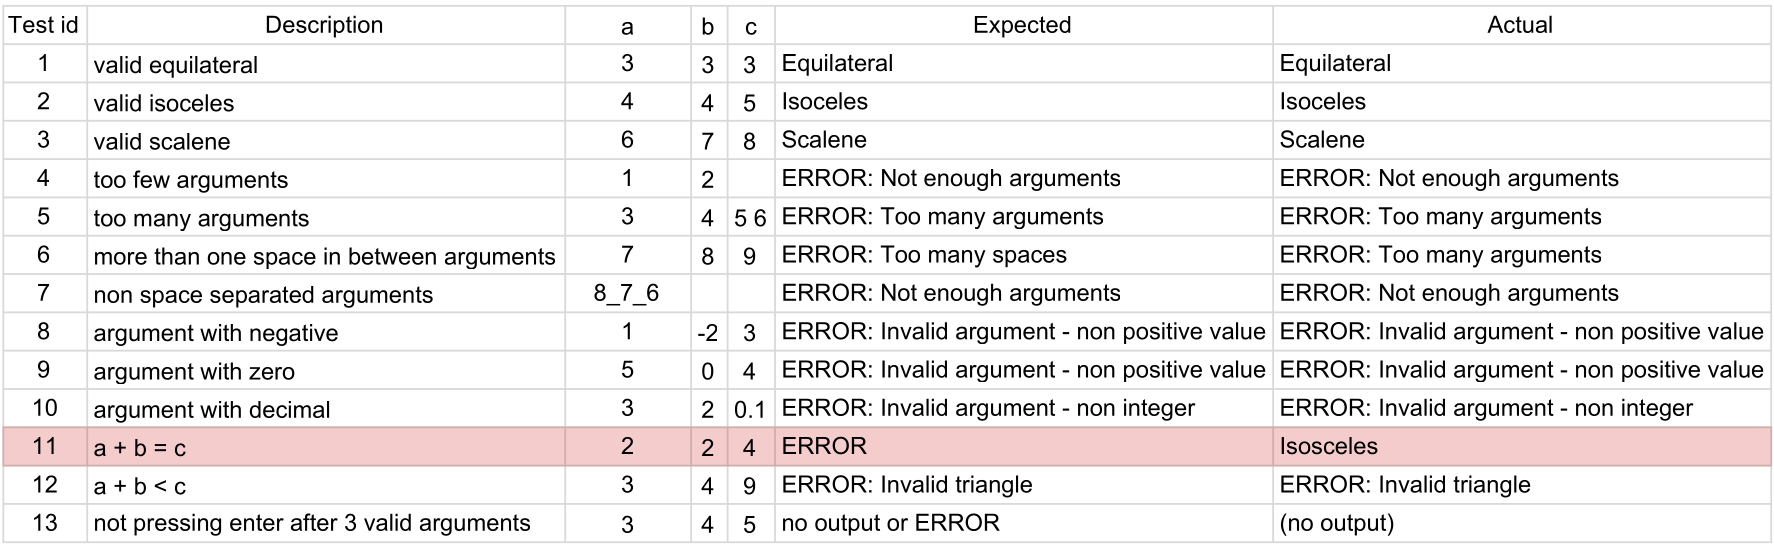
\includegraphics[width=1.1\textwidth]{triangletable.png}
    \end{figure}
    \caption{Test cases covering the equivalence classes identified in Part 2 for the Triangle program. Failed test cases are highlighted in red.}
\end{table}
\end{document}